\documentclass[handout]{beamer}
%\documentclass [serif,mathserif,professionalfont]{beamer}
%\usepackage {pxfonts}
%\usepackage {eulervm}
%\usepackage{mathpazo}
%\logo{\includegraphics[height=1.2cm]{fsulogo.png}}

\usepackage{tikz}
\usepackage{graphicx}
\usepackage{subfig,fixltx2e,url}
\usepackage[latin1]{inputenc}
\usepackage{pgfplots}
\usepackage{hyperref}
\usepackage{booktabs}

%\usetheme{Warsaw}
\usecolortheme{lily}
\setbeamercovered{transparent}
%\useoutertheme[subsection=false]{smoothbars}

\setbeamertemplate{sidebar right}{}
\setbeamertemplate{footline}{%
\hfill\usebeamertemplate***{navigation symbols}
\hspace{1cm}\insertframenumber{}/\inserttotalframenumber}

\title[ \insertdate]{Change Detection}

\author{Sagar Verma}
\institute[Granular AI] % (optional, but mostly needed)
{
24 Stony Brook Road
Belmont MA, 02478 USA}
% - Use the \inst command only if there are several affiliations.
% - Keep it simple, no one is interested in your street address.

\date{November, 2018}
% - Either use conference name or its abbreviation.
% - Not really informative to the audience, more for people (including

\begin{document}

\begin{frame}
\titlepage
\end{frame}

\begin{frame}{Table Of Contents}
\begin{enumerate}
\item Problem Statement
\item Background
\item Dataset and Experiments
\item Results and Conclusions
\end{enumerate}
\end{frame}

\section{Problem Statement}

\begin{frame}{Problem Statement}
\begin{center}
\begin{enumerate}
  \item Detect pixel wise change.
  \item Input: Multiple dates' images of same location.
  \item Output: Change mask between start and end dates.
\end{enumerate}
\vspace{.5cm}
  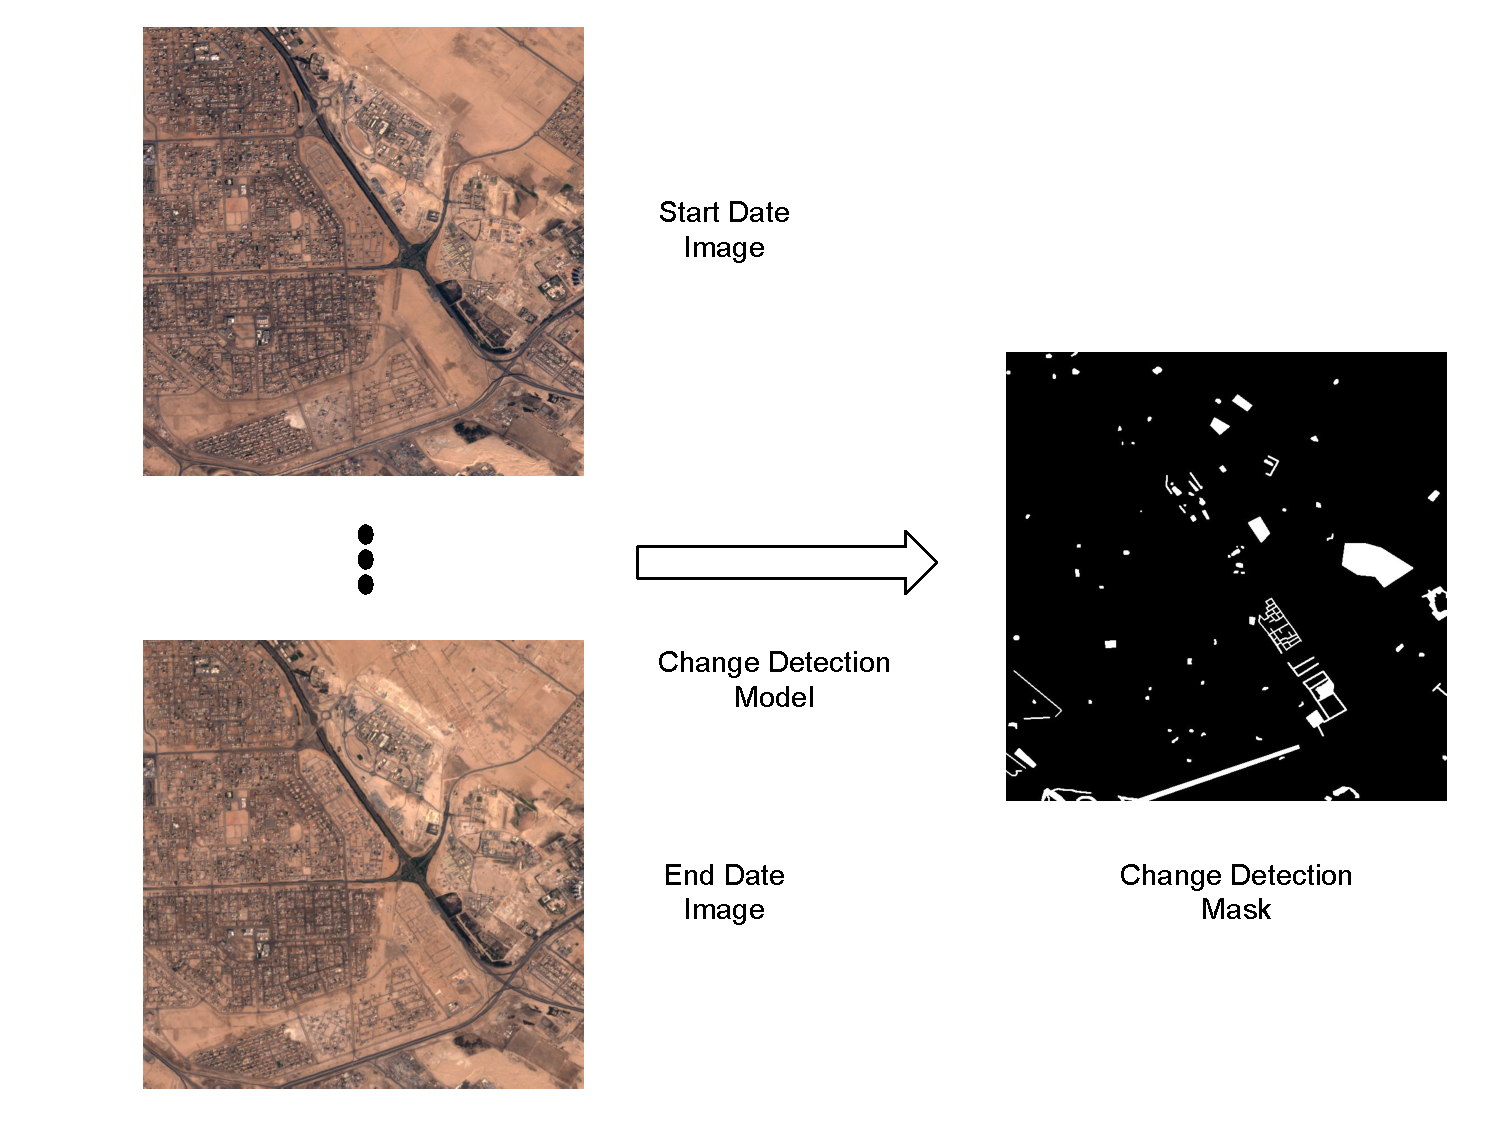
\includegraphics[scale=0.25]{images/cdteaser}
\end{center}
\end{frame}


\begin{frame}{Problem Statement}{Challenges}
  \begin{enumerate}
    \item How to handle multiple dates as input?
    \item Unsupervised model, if data scarcity?
    \item Supervised model, if data abundance?
    \item Evaluation criteria for change.
  \end{enumerate}
\end{frame}

\section{Background}
\begin{frame}{Background}
  \begin{enumerate}
    \item Recurrent Neural Networks
    \item Long-Short Term Memory
    \item 3D Convolution
  \end{enumerate}
\end{frame}

\begin{frame}{Background}{Recurrent Neural Networks}
  \begin{enumerate}
    \item Perform same task for every element of a sequence.
    \item Output depends on previous elements.
    \item RNNs can be seen as a neural network having "memory".
    \begin{equation}
        h_t = tanh(Wx_t+Uh_{t-1}),
    \end{equation}
    where $W$ and $U$ are weights, $h$ is the hidden vector and $x_t$ is the input at time $t$.
  \end{enumerate}
  \begin{center}
    \begin{figure}
    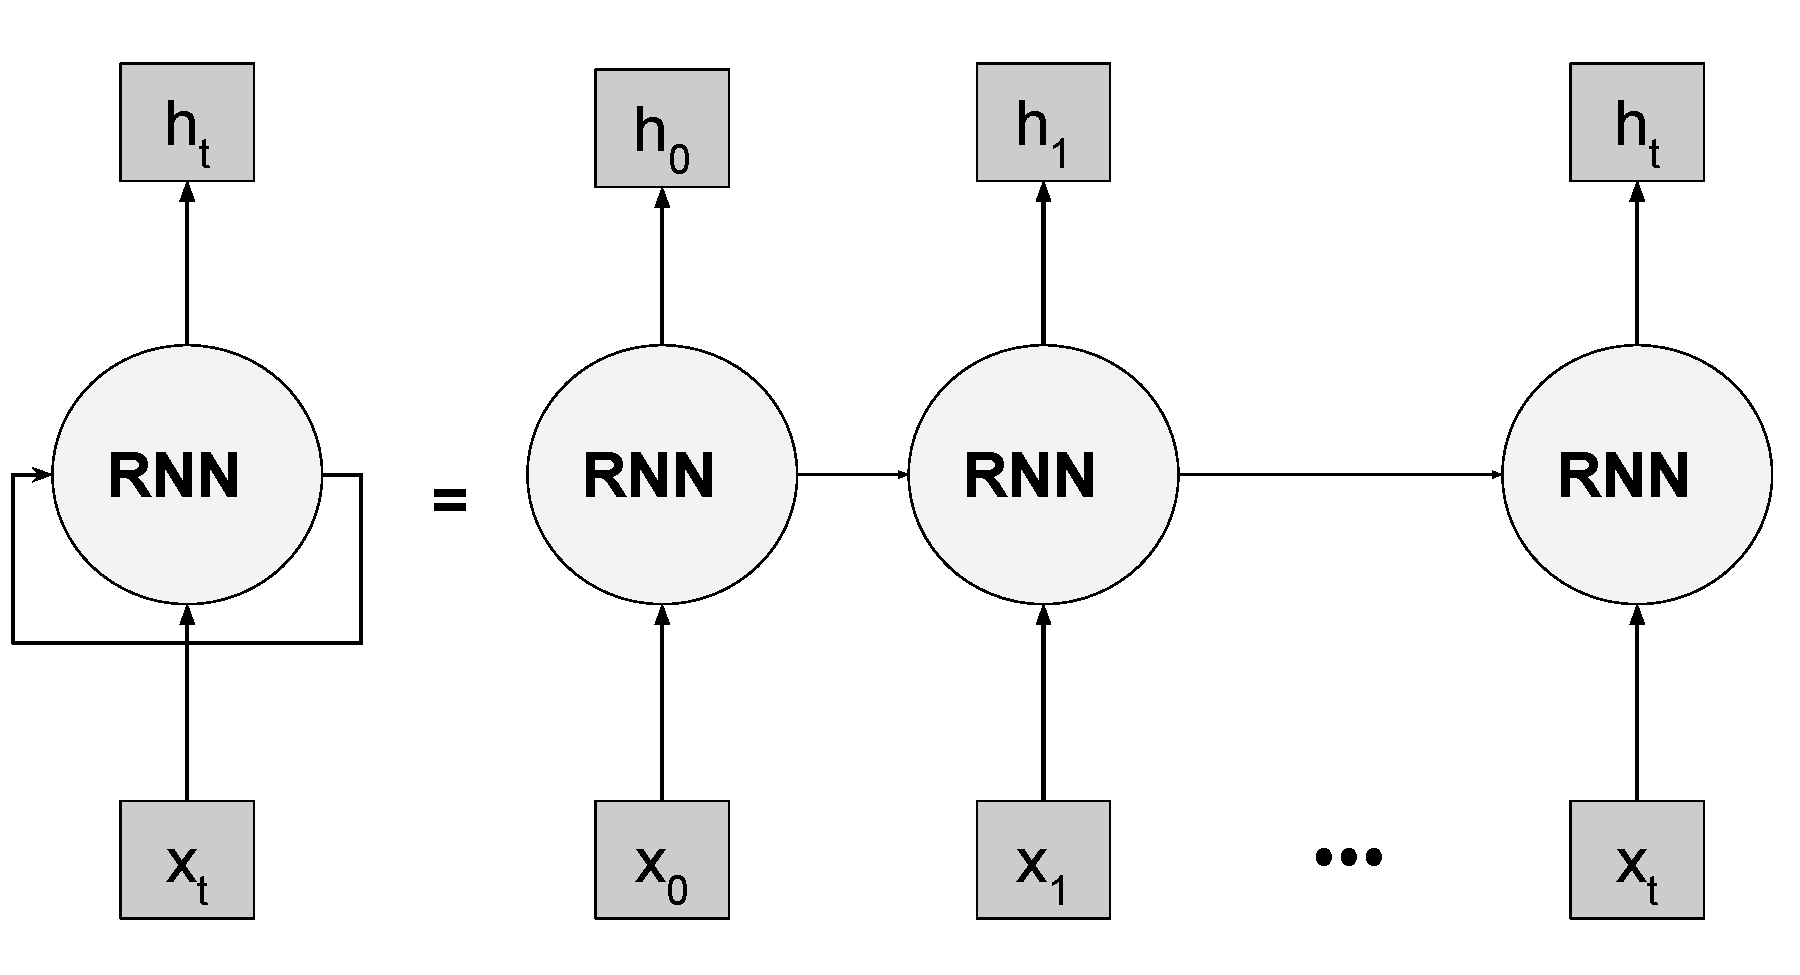
\includegraphics[width=0.6\linewidth, height=3.5cm]{images/RNN}
    \caption{RNN unrolled in time.}
    \end{figure}
  \end{center}
\end{frame}

\begin{frame}{Background}{Sequential Networks: Long-Short Term Memory}
  \begin{enumerate}
    \item RNNs have vanishing and exploding gradients problem.
    \item LSTM resolves above problems.
    \item Computes when to forget and when to remember.
  \end{enumerate}
  \begin{center}
    \begin{figure}
    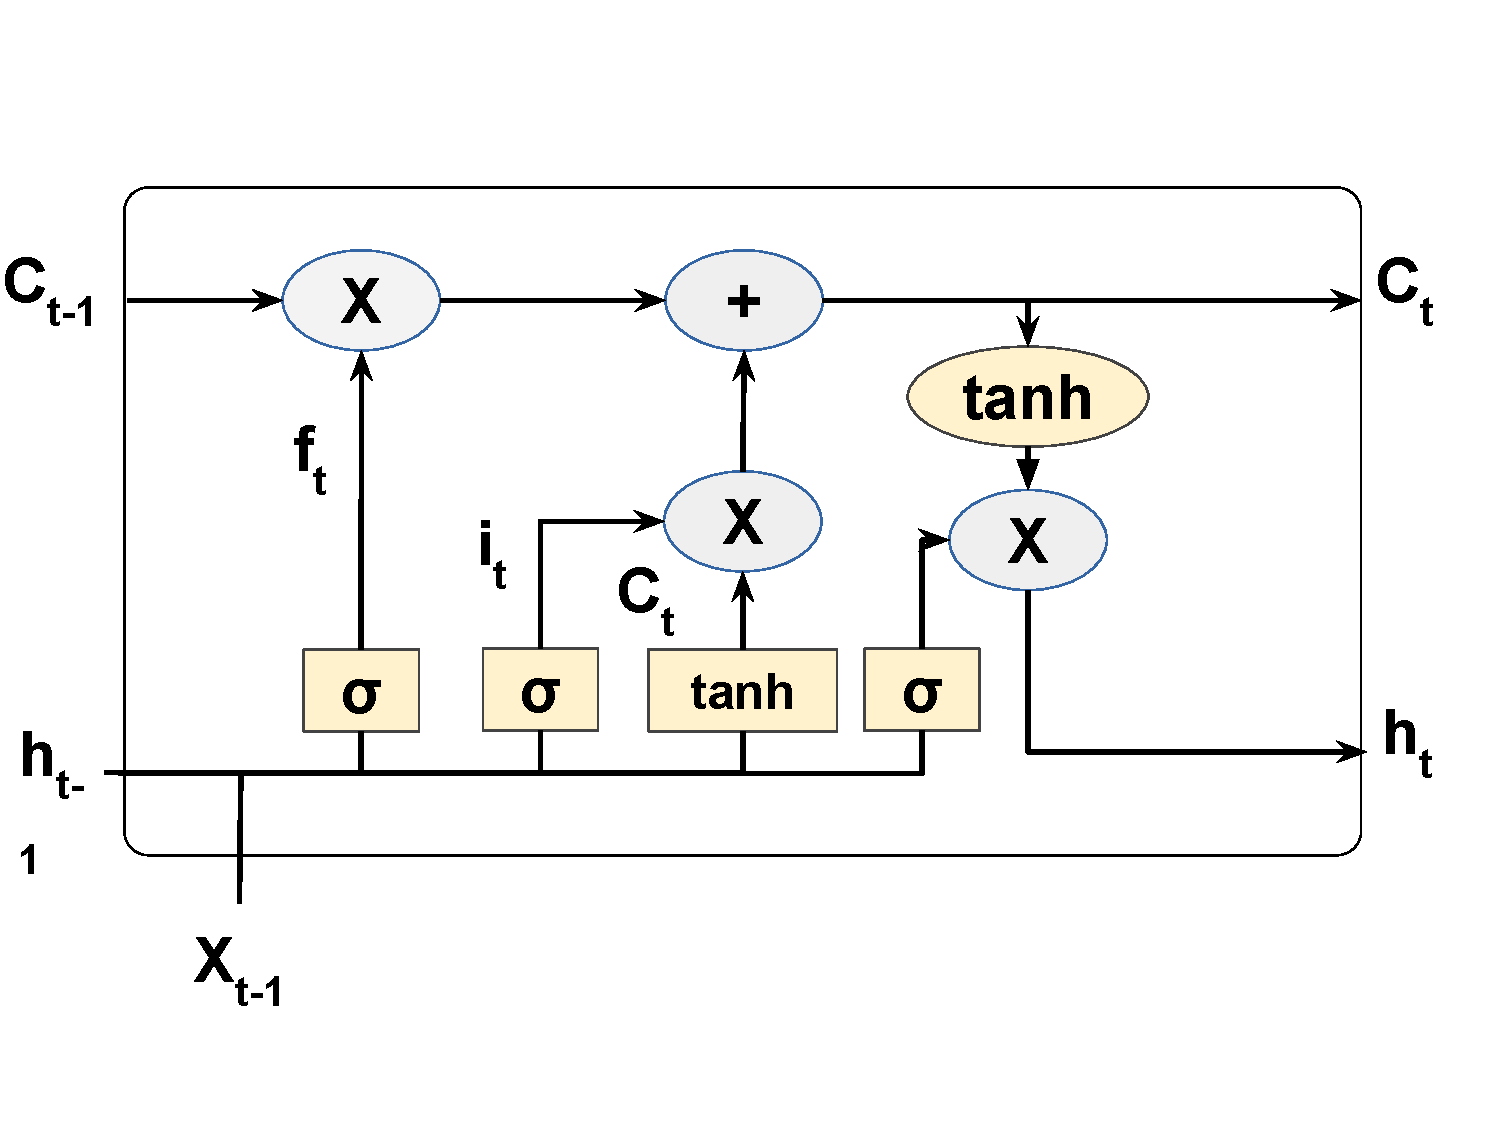
\includegraphics[width=0.6\linewidth, height=4cm]{images/lstm}
    \caption{LSTM Cell.}
    \end{figure}
  \end{center}
\end{frame}

\begin{frame}{3D Convolution}
  \begin{enumerate}
    \item 4D data, height, width, time/depth, and channel
    \item 3D kernel, 3D convolve operation
    \item Convolve along height, width and time/depth
    \item Used in video tasks and 3d medical images
  \end{enumerate}
  \begin{center}
    \begin{figure}
    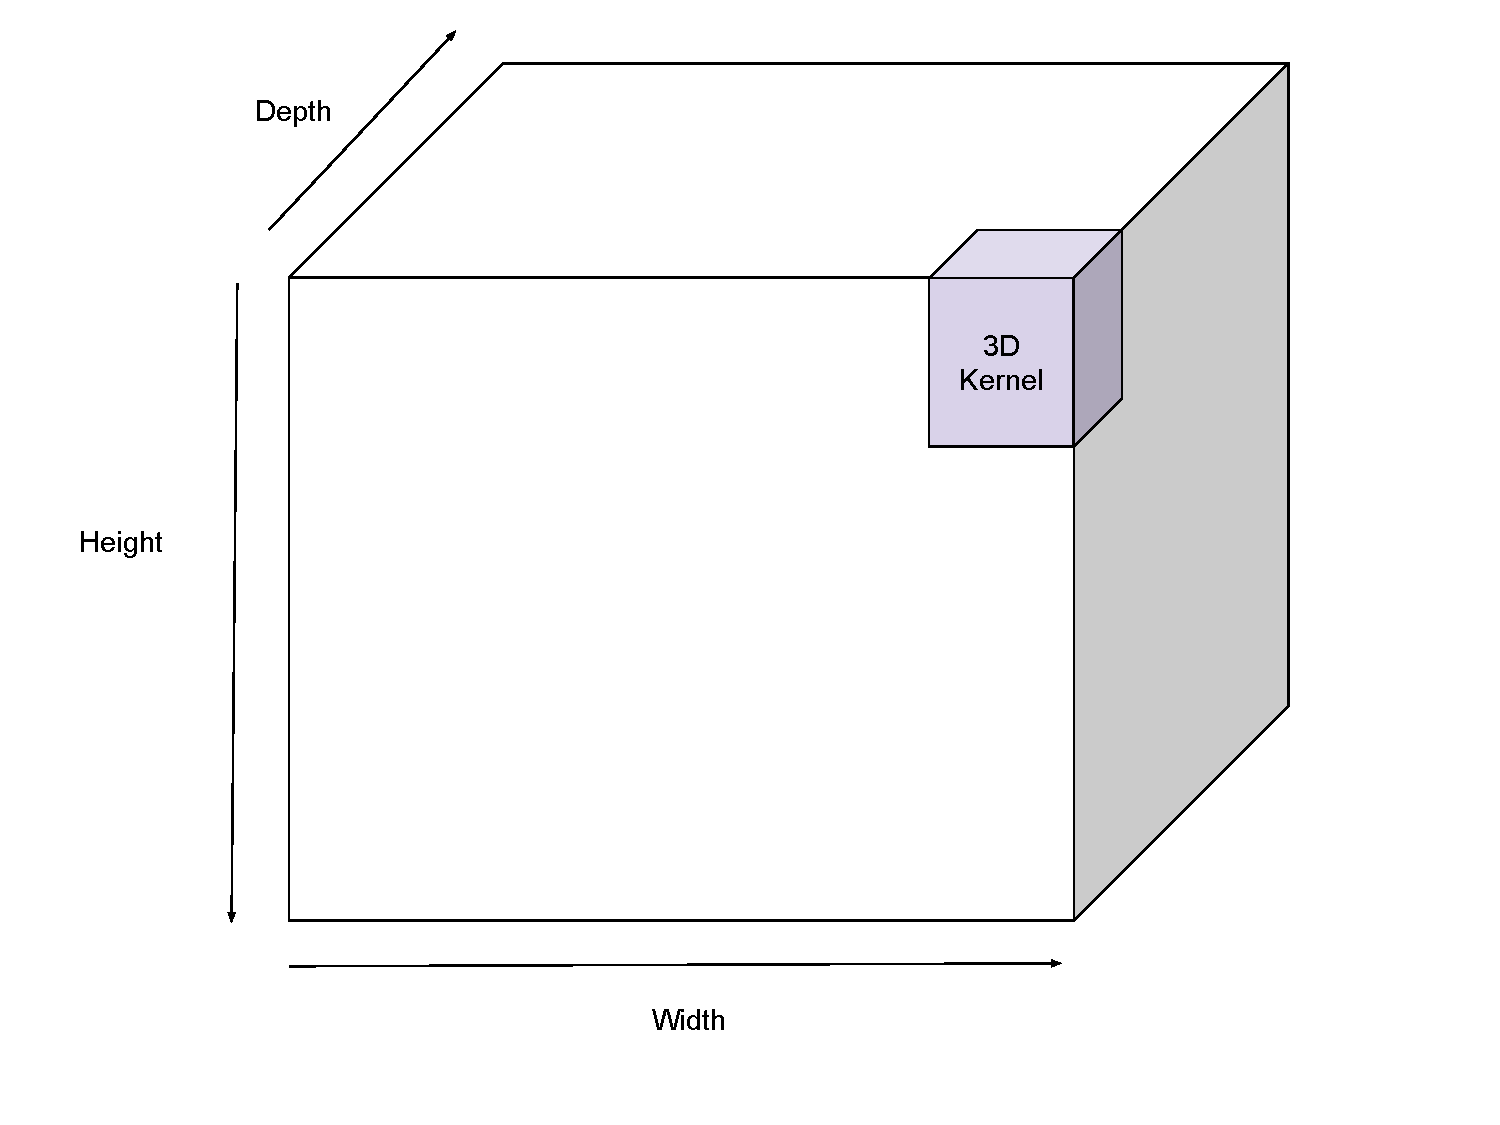
\includegraphics[width=0.6\linewidth, height=4cm]{images/3dconvolution}
    \caption{LSTM Cell.}
    \end{figure}
  \end{center}
\end{frame}

\section{Dataset}
\begin{frame}{Dataset and Experiments}{Dataset}
  \begin{enumerate}
    \item \href{https://rcdaudt.github.io/oscd/}{\color{blue}\textit{ONERA}} dataset.
    \item 24 locations through out world.
    \item Image pairs, two dates.
    \item 14 location for training, 10 for testing.
    \item 13 bands, sentinel data.
    \item Change mask, but everything reprojected.
  \end{enumerate}
\end{frame}

\begin{frame}{Dataset and Experiments}{Unsupervised Change Detection}
  \begin{enumerate}
    \item Multiple dates, single pixel as input.
    \item Try to reconstruct the input.
    \item If change occurs reconstruction error is high.
  \end{enumerate}
  \begin{center}
    \begin{figure}
    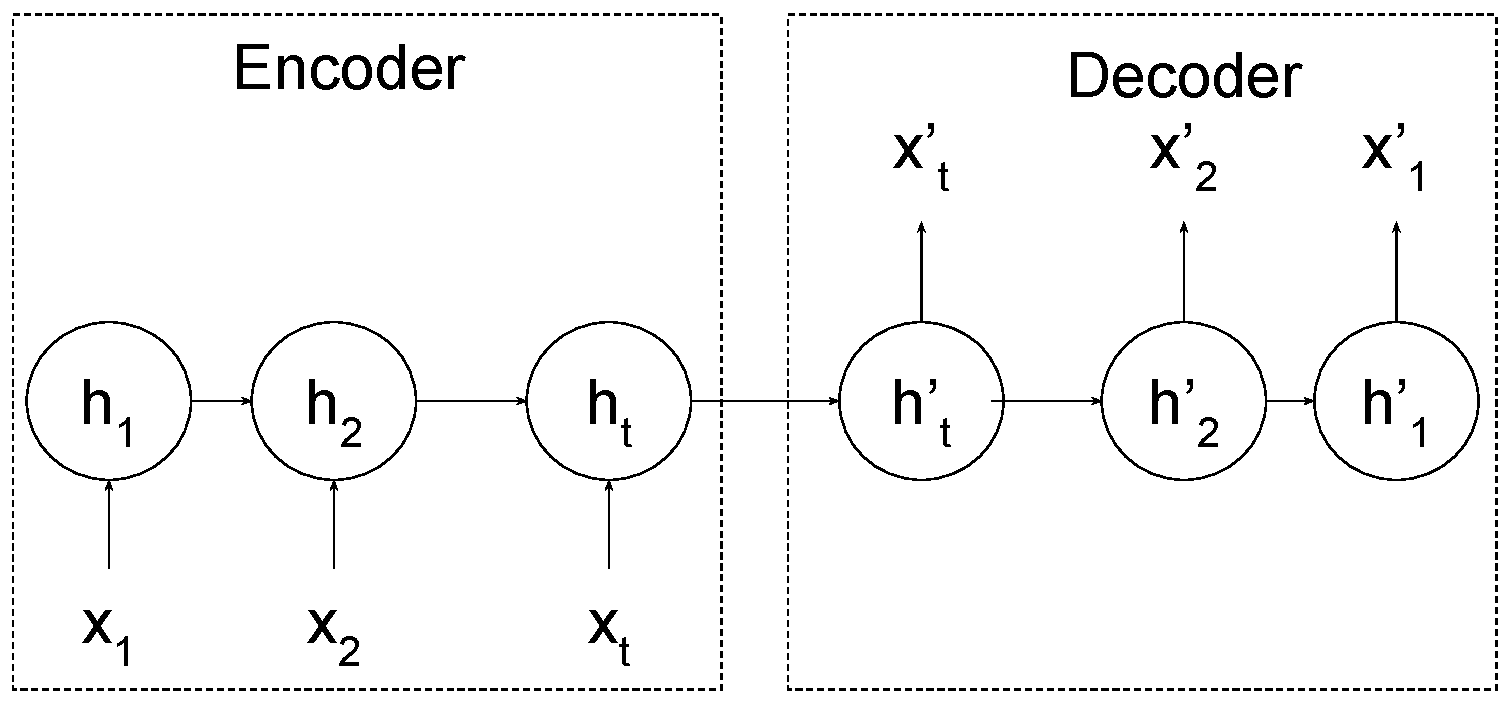
\includegraphics[scale=0.35]{images/rnn_enc_dec}
    \end{figure}
  \end{center}
\end{frame}

\begin{frame}{Dataset and Experiments}{Supervised Change Detection: 3D CNN}
  \begin{enumerate}
      \item Use labeled data, change mask.
      \item Stack multiple dates as input.
      \item Apply 3D convolution, then 2d convolution.
      \item SegNet like architecture.
  \end{enumerate}
  \begin{center}
    \begin{figure}
    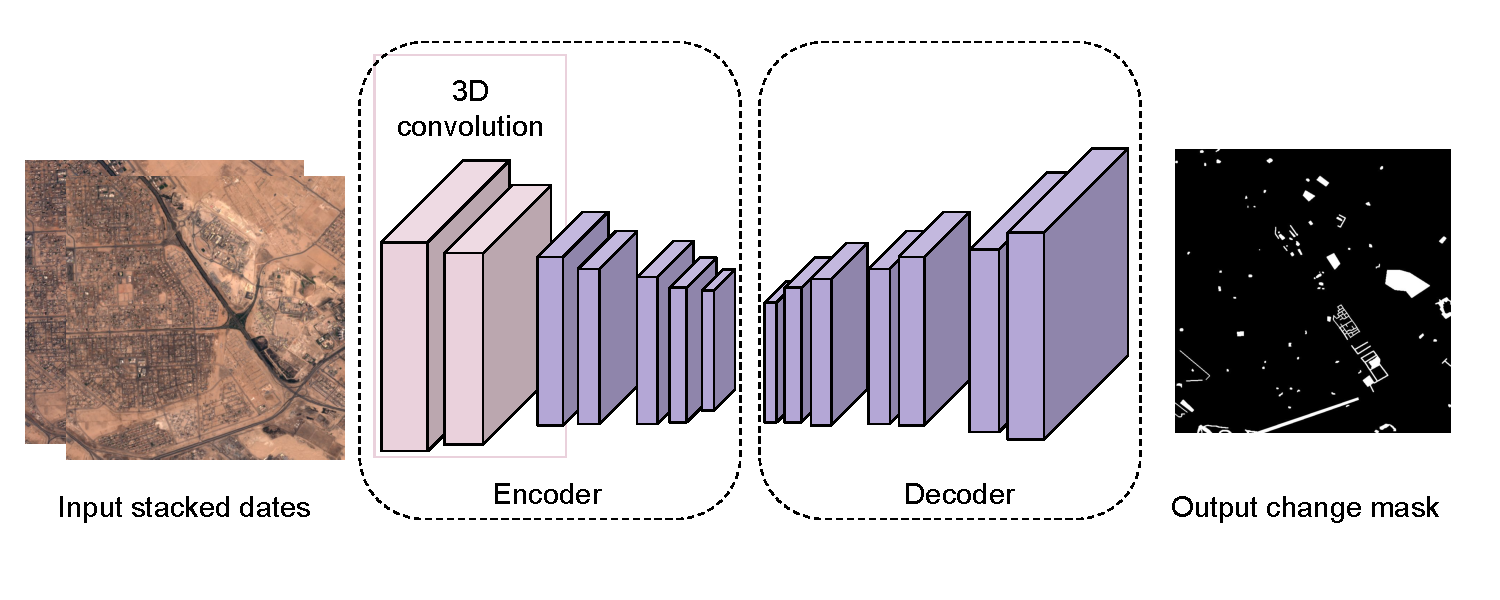
\includegraphics[scale=0.35]{images/3dconv_seg}
    \end{figure}
  \end{center}
\end{frame}


\begin{frame}{Results and Conclusions}{Model Convergence}

\end{frame}

\begin{frame}{Results and Conclusions}{Example Outputs}

\end{frame}

\section{Conclusions and Future Work}
\begin{frame}{Results and Conclusions}{}

\end{frame}

\begin{frame}
\center
\color{blue}
\huge{Thank you!}\\
\huge{Questions?}\\
\end{frame}

\end{document}
